% Topic T6.4: What's Next?
% Self-contained Beamer slides for Digital Finance course
\documentclass[11pt,aspectratio=169]{beamer}
\usetheme{Madrid}

% ======================= PACKAGES =======================
\usepackage{graphicx}
\usepackage{booktabs}
\usepackage{adjustbox}
\usepackage{multicol}
\usepackage{amsmath}
\usepackage{amssymb}
\usepackage{tikz}
\usetikzlibrary{arrows,shapes,positioning,shadows,trees}
\usepackage{listings}
\usepackage{xcolor}

% ======================= COLOR DEFINITIONS =======================
% Primary color scheme: Blue/Teal for Digital Finance
\definecolor{dfblue}{RGB}{0,102,204}
\definecolor{dfteal}{RGB}{0,153,153}
\definecolor{dfcyan}{RGB}{51,187,204}
\definecolor{dflightblue}{RGB}{153,204,255}
\definecolor{dflightblue2}{RGB}{173,214,255}
\definecolor{dflightblue3}{RGB}{193,224,255}
\definecolor{dflightblue4}{RGB}{213,234,255}

% Accent colors for finance applications
\definecolor{dfgreen}{RGB}{44, 160, 44}
\definecolor{dfred}{RGB}{214, 39, 40}
\definecolor{dforange}{RGB}{255, 127, 14}
\definecolor{dfgray}{RGB}{127, 127, 127}

% Utility colors
\definecolor{lightgray}{RGB}{240, 240, 240}
\definecolor{midgray}{RGB}{180, 180, 180}
\definecolor{codebg}{RGB}{245, 245, 245}

% ======================= THEME CUSTOMIZATION =======================
% Apply Digital Finance color scheme to Madrid theme
\setbeamercolor{palette primary}{bg=dflightblue3,fg=dfblue}
\setbeamercolor{palette secondary}{bg=dflightblue2,fg=dfblue}
\setbeamercolor{palette tertiary}{bg=dfteal,fg=white}
\setbeamercolor{palette quaternary}{bg=dfblue,fg=white}

\setbeamercolor{structure}{fg=dfblue}
\setbeamercolor{section in toc}{fg=dfblue}
\setbeamercolor{subsection in toc}{fg=dfteal}
\setbeamercolor{title}{fg=dfblue}
\setbeamercolor{frametitle}{fg=dfblue,bg=dflightblue3}
\setbeamercolor{block title}{bg=dflightblue2,fg=dfblue}
\setbeamercolor{block body}{bg=dflightblue4,fg=black}

% Remove navigation symbols for cleaner look
\setbeamertemplate{navigation symbols}{}

% Clean itemize/enumerate
\setbeamertemplate{itemize items}[circle]
\setbeamertemplate{enumerate items}[default]

% Margins for readability
\setbeamersize{text margin left=8mm,text margin right=8mm}

% ======================= LISTINGS CONFIGURATION =======================
% Python code style
\lstdefinestyle{pythonstyle}{
    language=Python,
    basicstyle=\ttfamily\footnotesize,
    keywordstyle=\color{dfblue}\bfseries,
    stringstyle=\color{dforange},
    commentstyle=\color{dfgray}\itshape,
    numberstyle=\tiny\color{dfgray},
    numbers=left,
    numbersep=5pt,
    backgroundcolor=\color{codebg},
    showspaces=false,
    showstringspaces=false,
    showtabs=false,
    frame=single,
    rulecolor=\color{midgray},
    tabsize=4,
    captionpos=b,
    breaklines=true,
    breakatwhitespace=false,
    escapeinside={(*@}{@*)},
    xleftmargin=10pt,
    xrightmargin=10pt
}

% Solidity code style
\lstdefinestyle{soliditystyle}{
    language=Java, % closest approximation
    basicstyle=\ttfamily\footnotesize,
    keywordstyle=\color{dfteal}\bfseries,
    stringstyle=\color{dforange},
    commentstyle=\color{dfgray}\itshape,
    numberstyle=\tiny\color{dfgray},
    numbers=left,
    numbersep=5pt,
    backgroundcolor=\color{codebg},
    showspaces=false,
    showstringspaces=false,
    showtabs=false,
    frame=single,
    rulecolor=\color{midgray},
    tabsize=2,
    captionpos=b,
    breaklines=true,
    breakatwhitespace=false,
    escapeinside={(*@}{@*)},
    xleftmargin=10pt,
    xrightmargin=10pt,
    morekeywords={pragma, contract, function, returns, public, private, view, pure, payable, address, uint256, mapping, event, modifier}
}

% Inline code command
\newcommand{\code}[1]{\texttt{\color{dfblue}#1}}

% ======================= CUSTOM COMMANDS =======================
% Bottom annotation (Madrid-style)
\newcommand{\bottomnote}[1]{%
\vfill
\vspace{-2mm}
\textcolor{dflightblue2}{\rule{\textwidth}{0.4pt}}
\vspace{1mm}
\footnotesize
\textbf{#1}
}

% Compact list spacing
\newcommand{\compactlist}{%
\setlength{\itemsep}{0pt}%
\setlength{\parskip}{0pt}%
\setlength{\parsep}{0pt}%
}

% Chart placeholder
\newcommand{\chartplaceholder}[2][5cm]{%
\begin{center}
\begin{adjustbox}{max width=0.95\textwidth, max height=#1}
\framebox[\textwidth][c]{%
\rule{0pt}{#1}%
\textcolor{midgray}{[#2]}%
}
\end{adjustbox}
\end{center}
}

% ======================= FINANCE NOTATION MACROS =======================
% Probability and statistics
\newcommand{\E}{\mathbb{E}} % Expected value
\newcommand{\Var}{\mathrm{Var}} % Variance
\newcommand{\Cov}{\mathrm{Cov}} % Covariance
\newcommand{\Prob}{\mathbb{P}} % Probability

% Distributions
\newcommand{\Normal}{\mathcal{N}} % Normal distribution
\newcommand{\Uniform}{\mathcal{U}} % Uniform distribution

% Returns and prices
\newcommand{\Ret}{R} % Return
\newcommand{\LogRet}{r} % Log return
\newcommand{\Price}{S} % Price/Stock price
\newcommand{\Strike}{K} % Strike price

% Options and derivatives
\newcommand{\CallPrice}{C} % Call option price
\newcommand{\PutPrice}{P} % Put option price
\newcommand{\Greeks}[1]{\mathit{#1}} % Greek letters

% Risk measures
\newcommand{\VaR}{\mathrm{VaR}} % Value at Risk
\newcommand{\CVaR}{\mathrm{CVaR}} % Conditional VaR
\newcommand{\Sharpe}{\mathrm{SR}} % Sharpe Ratio

% Time series
\newcommand{\AR}{\mathrm{AR}} % Autoregressive
\newcommand{\MA}{\mathrm{MA}} % Moving average
\newcommand{\GARCH}{\mathrm{GARCH}} % GARCH

% Blockchain/Crypto
\newcommand{\Hash}{\mathrm{Hash}} % Hash function
\newcommand{\Block}{\mathcal{B}} % Block
\newcommand{\Chain}{\mathcal{C}} % Chain

% Real numbers, integers
\newcommand{\R}{\mathbb{R}}
\newcommand{\Z}{\mathbb{Z}}
\newcommand{\N}{\mathbb{N}}

% ======================= TIKZ STYLES =======================
% Styles for finance-related diagrams
\tikzstyle{process} = [rectangle, minimum width=3cm, minimum height=1cm, text centered, draw=dfblue, fill=dflightblue4, thick]
\tikzstyle{decision} = [diamond, minimum width=3cm, minimum height=1cm, text centered, draw=dfteal, fill=dflightblue4, thick]
\tikzstyle{arrow} = [thick,->,>=stealth,color=dfblue]
\tikzstyle{blockchain} = [rectangle, rounded corners, minimum width=2.5cm, minimum height=1cm, text centered, draw=dfteal, fill=dflightblue3, thick]
\tikzstyle{transaction} = [circle, minimum size=0.8cm, text centered, draw=dforange, fill=dflightblue4, thick]

% ======================= FOOTER TEMPLATE =======================
\setbeamertemplate{footline}{
    \hbox{\begin{beamercolorbox}[wd=\paperwidth,ht=2.5ex,dp=1ex,leftskip=.5em,rightskip=.5em]{author in head/foot}
    \tiny
    \textbf{Digital Finance} \hfill
    Joerg Osterrieder \hfill
    \insertdate \hfill
    Page \insertframenumber{} / \inserttotalframenumber
    \end{beamercolorbox}}
}

% ======================= SECTION DIVIDER TEMPLATE =======================
\AtBeginSection[]{
\begin{frame}[plain]
\vfill
\centering
\begin{beamercolorbox}[sep=12pt,center]{title}
\usebeamerfont{title}\LARGE\insertsection\par
\end{beamercolorbox}
\vfill
\end{frame}
}


\title[T6.4: What's Next?]{Topic 6.4: What's Next?}
\subtitle{The Future of Digital Finance}
\author{Joerg Osterrieder}
\institute{Digital Finance}
\date{2026}

\begin{document}

% =============================================================================
% Frame 1: Title Slide
% =============================================================================
\begin{frame}[plain]
\titlepage
\end{frame}

% =============================================================================
% Frame 2: Learning Objectives
% =============================================================================
\begin{frame}{Learning Objectives}
\begin{center}
\textbf{\Large What You Will Learn in This Topic}
\end{center}

\vspace{5mm}
By the end of this session, you will be able to:

\begin{enumerate}
\item \textbf{Identify} the genuinely open questions shaping digital finance's next decade
\item \textbf{Analyze} the interoperability debate and future chain architectures
\item \textbf{Evaluate} the CBDC vs. private digital money landscape
\item \textbf{Understand} emerging threats from quantum computing and AI
\item \textbf{Develop} informed hypotheses about the future of money
\item \textbf{Synthesize} key learnings from the entire course
\end{enumerate}

\vspace{5mm}
\begin{block}{Course Finale}
This is the concluding topic of Digital Finance. We look forward while consolidating everything learned.
\end{block}
\end{frame}

% =============================================================================
% Frame 3: Prerequisites/Background I
% =============================================================================
\begin{frame}{Prerequisites: Building on Everything}
\begin{columns}[T]
\begin{column}{0.48\textwidth}
\textbf{What you should know:}
\begin{itemize}
\item Digital payments and FinTech (Day 2)
\item Blockchain fundamentals (Day 3)
\item Smart contracts and DeFi (Day 4)
\item Stablecoins and tokenization (Day 4)
\item Regulatory frameworks (Day 5)
\item Convergence thesis (Day 6)
\end{itemize}

\vspace{3mm}
\textbf{Key concepts to recall:}
\begin{itemize}
\item Consensus mechanisms
\item Layer 1 vs. Layer 2 scaling
\item CBDC architectures
\item AI in finance applications
\end{itemize}
\end{column}
\begin{column}{0.48\textwidth}
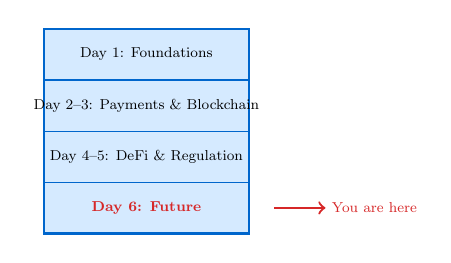
\begin{tikzpicture}[scale=0.65, transform shape]
% Knowledge progression
\draw[thick, dfblue, fill=dflightblue4] (0,0) rectangle (4,4);
\node at (2,3.5) {\footnotesize Day 1: Foundations};
\draw[dfblue] (0,3) -- (4,3);
\node at (2,2.5) {\footnotesize Day 2--3: Payments \& Blockchain};
\draw[dfblue] (0,2) -- (4,2);
\node at (2,1.5) {\footnotesize Day 4--5: DeFi \& Regulation};
\draw[dfblue] (0,1) -- (4,1);
\node[text=dfred] at (2,0.5) {\footnotesize \textbf{Day 6: Future}};

% Arrow
\draw[thick, dfred, ->] (4.5,0.5) -- (5.5,0.5);
\node[right] at (5.5,0.5) {\textcolor{dfred}{\footnotesize You are here}};
\end{tikzpicture}
\end{column}
\end{columns}
\end{frame}

% =============================================================================
% Frame 4: Prerequisites/Background II
% =============================================================================
\begin{frame}{The Big Picture: Why ``What's Next'' Matters}
\begin{center}
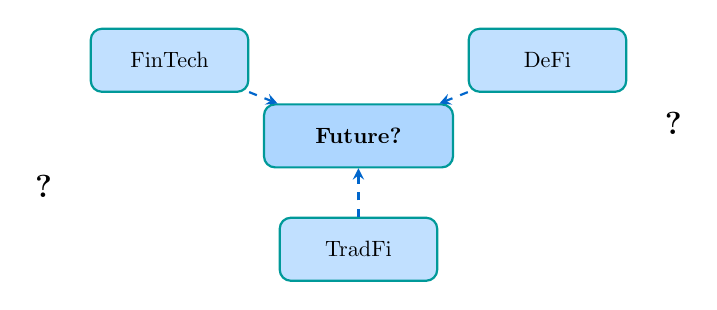
\begin{tikzpicture}[scale=0.8, transform shape]
% Three spheres converging
\node[blockchain, minimum width=2.5cm] (fintech) at (-3,2) {FinTech};
\node[blockchain, minimum width=2.5cm] (defi) at (3,2) {DeFi};
\node[blockchain, minimum width=2.5cm] (tradfi) at (0,-1) {TradFi};

% Convergence point
\node[blockchain, fill=dflightblue2, minimum width=3cm] (future) at (0,0.8) {\textbf{Future?}};

% Arrows
\draw[arrow, dashed] (fintech) -- (future);
\draw[arrow, dashed] (defi) -- (future);
\draw[arrow, dashed] (tradfi) -- (future);

% Question marks
\node at (5,1) {\Large \textbf{?}};
\node at (-5,0) {\Large \textbf{?}};
\end{tikzpicture}
\end{center}

\vspace{3mm}
\textbf{The honest answer:} We don't know exactly what the future holds.

\vspace{2mm}
\textbf{But we can identify:}
\begin{itemize}
\item The genuinely open questions that will shape outcomes
\item The forces and trends likely to matter
\item The frameworks for thinking about any future development
\end{itemize}
\end{frame}

% =============================================================================
% Frame 5: The Genuinely Open Questions
% =============================================================================
\begin{frame}{The Genuinely Open Questions}
\begin{block}{These questions will shape the next decade of digital finance:}
\end{block}

\begin{enumerate}
\item \textbf{Interoperability}: Will we see one dominant chain, many chains, or seamless cross-chain?
\item \textbf{CBDC vs. Private Money}: Will central bank digital currencies dominate, or coexist with stablecoins?
\item \textbf{Decentralized Identity}: Will blockchain-based identity systems achieve adoption?
\item \textbf{Quantum Threats}: How will cryptography adapt to quantum computing?
\item \textbf{AI Autonomy}: Will AI agents hold assets and transact independently?
\item \textbf{Regulatory Equilibrium}: Where will global regulation settle?
\item \textbf{The Future of Money}: What \emph{is} money in 2035?
\end{enumerate}
\end{frame}

% =============================================================================
% Frame 6: Open Question: Interoperability - Current State
% =============================================================================
\begin{frame}{Open Question: Interoperability}
\begin{columns}[T]
\begin{column}{0.48\textwidth}
\textbf{Current State:}
\begin{itemize}
\item Multiple Layer 1 chains (Ethereum, Solana, etc.)
\item Multiple Layer 2s (Layer 1 is the main blockchain; Layer 2 is a faster layer built on top: Arbitrum, Optimism, Base)
\item Fragmented liquidity
\item Bridge vulnerabilities (\$2B+ hacked cumulative, 2020--2023)
\item Poor user experience
\end{itemize}
\end{column}
\begin{column}{0.48\textwidth}
\textbf{Possible Futures:}
\begin{itemize}
\item \textbf{One chain wins}: Network effects concentrate
\item \textbf{Chain abstraction}: Users don't know/care which chain
\item \textbf{Specialized chains}: Different chains for different uses
\item \textbf{Traditional wins}: Banks don't need public chains
\end{itemize}
\end{column}
\end{columns}

\vspace{0.3cm}
\begin{block}{Discussion Question}
Is the future of blockchain ``one chain to rule them all'' or an interoperable multi-chain world? What are the arguments for each?
\end{block}
\end{frame}

% =============================================================================
% Frame 7: Interoperability - Technical Challenges
% =============================================================================
\begin{frame}{Interoperability: Technical Deep Dive}
\begin{center}
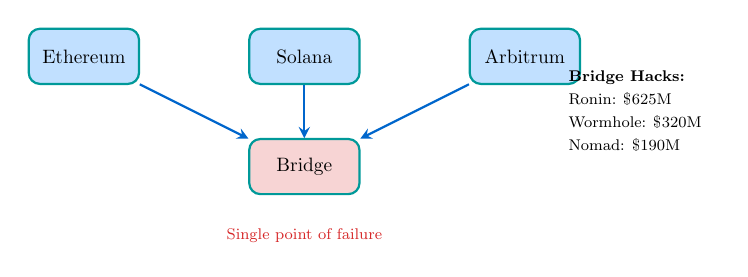
\begin{tikzpicture}[scale=0.7, transform shape]
% Multiple chains
\node[blockchain, minimum width=2cm] (eth) at (-4,2) {Ethereum};
\node[blockchain, minimum width=2cm] (sol) at (0,2) {Solana};
\node[blockchain, minimum width=2cm] (arb) at (4,2) {Arbitrum};

% Bridge in the middle
\node[blockchain, fill=dfred!20, minimum width=2cm] (bridge) at (0,0) {Bridge};

% Connections
\draw[arrow] (eth) -- (bridge);
\draw[arrow] (sol) -- (bridge);
\draw[arrow] (arb) -- (bridge);

% Warning
\node[below] at (0,-1) {\textcolor{dfred}{\footnotesize Single point of failure}};

% Stats
\node at (6,1) {
\begin{tabular}{l}
\footnotesize \textbf{Bridge Hacks:}\\
\footnotesize Ronin: \$625M\\
\footnotesize Wormhole: \$320M\\
\footnotesize Nomad: \$190M
\end{tabular}
};
\end{tikzpicture}
\end{center}

\vspace{3mm}
\textbf{The Bridge Trilemma:}
\begin{itemize}
\item \textbf{Security}: Minimizing trust assumptions
\item \textbf{Speed}: Fast finality across chains
\item \textbf{Generalizability}: Works for any chain pair
\end{itemize}

\begin{alertblock}{Current Reality}
Most bridges sacrifice security for speed and generalizability, creating systemic risk.
\end{alertblock}
\end{frame}

% =============================================================================
% Frame 8: CBDCs vs. Private Digital Money
% =============================================================================
\begin{frame}{Open Question: CBDCs vs. Private Digital Money}
\begin{columns}[T]
\begin{column}{0.48\textwidth}
\textbf{Arguments for CBDCs:}
\begin{itemize}
\item Central bank backing = safe
\item Monetary policy transmission
\item Financial inclusion
\item Reduced settlement risk
\item Programmable policy tools
\end{itemize}

\vspace{0.2cm}
\textbf{Status:} 130+ countries exploring (source: Atlantic Council CBDC Tracker, 2024); China, Nigeria, Bahamas live
\end{column}
\begin{column}{0.48\textwidth}
\textbf{Arguments for Private Money:}
\begin{itemize}
\item Innovation at the edge
\item Competition improves quality
\item Privacy from government
\item Borderless by design
\item Decentralization values
\end{itemize}

\vspace{0.2cm}
\textbf{Stablecoin market cap:} \$230B+ (as of late 2024)
\end{column}
\end{columns}

\vspace{0.3cm}
\begin{alertblock}{The Coexistence Hypothesis}
Most likely: CBDCs for domestic retail, regulated stablecoins for crypto/DeFi, and continued competition between payment systems.
\end{alertblock}
\end{frame}

% =============================================================================
% Frame 9: CBDC Implementation Models
% =============================================================================
\begin{frame}{CBDC Implementation Models}
\begin{center}
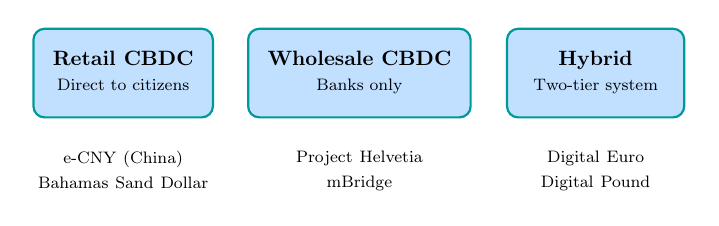
\begin{tikzpicture}[scale=0.75, transform shape]
% Three models
\node[blockchain, minimum width=3cm, minimum height=1.5cm] (retail) at (-4,0) {
\begin{tabular}{c}
\textbf{Retail CBDC}\\
\footnotesize Direct to citizens
\end{tabular}
};

\node[blockchain, minimum width=3cm, minimum height=1.5cm] (wholesale) at (0,0) {
\begin{tabular}{c}
\textbf{Wholesale CBDC}\\
\footnotesize Banks only
\end{tabular}
};

\node[blockchain, minimum width=3cm, minimum height=1.5cm] (hybrid) at (4,0) {
\begin{tabular}{c}
\textbf{Hybrid}\\
\footnotesize Two-tier system
\end{tabular}
};

% Labels below
\node[below, text width=3cm, align=center] at (-4,-1.2) {\footnotesize e-CNY (China)\\Bahamas Sand Dollar};
\node[below, text width=3cm, align=center] at (0,-1.2) {\footnotesize Project Helvetia\\mBridge};
\node[below, text width=3cm, align=center] at (4,-1.2) {\footnotesize Digital Euro\\Digital Pound};
\end{tikzpicture}
\end{center}

\vspace{5mm}
\begin{columns}[T]
\begin{column}{0.48\textwidth}
\textbf{Privacy Spectrum:}
\begin{itemize}
\item Full anonymity (cash-like)
\item Tiered limits (small = anonymous)
\item Full transparency (all tracked)
\end{itemize}
\end{column}
\begin{column}{0.48\textwidth}
\textbf{Design Choices:}
\begin{itemize}
\item Token vs. account-based
\item Interest-bearing or not
\item Programmable features
\end{itemize}
\end{column}
\end{columns}
\end{frame}

% =============================================================================
% Frame 10: Open Question: Decentralized Identity
% =============================================================================
\begin{frame}{Open Question: Decentralized Identity}
\begin{block}{The Problem}
Online identity today is fragmented, insecure, and controlled by platforms. Can blockchain fix this?
\end{block}

\begin{columns}[T]
\begin{column}{0.48\textwidth}
\textbf{DID/SSI Vision (Self-Sovereign Identity / Decentralized Identifiers --- letting individuals control their own digital identity):}
\begin{itemize}
\item Self-sovereign identity
\item User controls their data
\item Selective disclosure
\item Portable across platforms
\item Verifiable credentials
\end{itemize}
\end{column}
\begin{column}{0.48\textwidth}
\textbf{Challenges:}
\begin{itemize}
\item Key management for everyday users
\item Recovery when keys lost
\item Adoption chicken-and-egg
\item Regulatory acceptance
\item Competition from Big Tech
\end{itemize}
\end{column}
\end{columns}

\vspace{0.3cm}
\textbf{Watch:} EU eIDAS 2.0 (the EU's electronic identification and trust services regulation), Worldcoin (iris-scanning identity verification project), ENS (Ethereum Name Service --- human-readable blockchain addresses), Soulbound tokens (digital credentials that cannot be transferred, like a diploma), Polygon ID (privacy-preserving identity toolkit)
\end{frame}

% =============================================================================
% Frame 11: Open Question: Quantum Computing Threats
% =============================================================================
\begin{frame}{Open Question: Quantum Computing Threats}
\begin{columns}[T]
\begin{column}{0.48\textwidth}
\textbf{What's at Risk:}
\begin{itemize}
\item ECDSA (Elliptic Curve Digital Signature Algorithm --- the math that secures blockchain signatures, used by Bitcoin, Ethereum)
\item RSA (a widely used encryption algorithm)
\item Current digital signatures
\item Potentially: all historical transactions
\end{itemize}

\vspace{0.2cm}
\textbf{``Harvest Now, Decrypt Later''}: Adversaries may be storing encrypted data to break when quantum arrives.
\end{column}
\begin{column}{0.48\textwidth}
\textbf{Mitigation Paths:}
\begin{itemize}
\item Post-quantum cryptography (NIST standards)
\item Hash-based signatures (already quantum-resistant)
\item Migration plans for blockchains
\item Timeline uncertainty (10--30 years? Experts disagree widely on timing, but NIST has already begun standardizing post-quantum cryptography.)
\end{itemize}

\vspace{0.2cm}
\textbf{Good news:} Most blockchain systems can upgrade signature schemes.
\end{column}
\end{columns}
\end{frame}

% =============================================================================
% Frame 12: Quantum Timeline and Preparation
% =============================================================================
\begin{frame}{Quantum: Timeline and Preparation}
\begin{center}
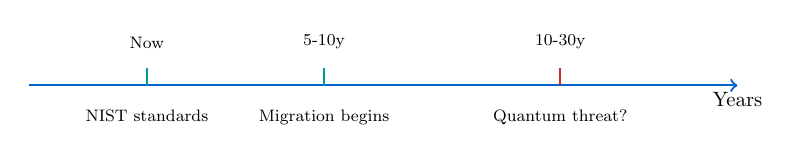
\begin{tikzpicture}[scale=0.75, transform shape]
% Timeline
\draw[thick, dfblue, ->] (0,0) -- (12,0);
\node[below] at (12,0) {Years};

% Markers
\draw[thick, dfteal] (2,0) -- (2,0.3);
\node[above] at (2,0.5) {\footnotesize Now};
\node[below] at (2,-0.3) {\footnotesize NIST standards};

\draw[thick, dfteal] (5,0) -- (5,0.3);
\node[above] at (5,0.5) {\footnotesize 5-10y};
\node[below] at (5,-0.3) {\footnotesize Migration begins};

\draw[thick, dfred] (9,0) -- (9,0.3);
\node[above] at (9,0.5) {\footnotesize 10-30y};
\node[below] at (9,-0.3) {\footnotesize Quantum threat?};
\end{tikzpicture}
\end{center}

\vspace{5mm}
\textbf{Post-Quantum Cryptography:}
In 2024, NIST (the US National Institute of Standards and Technology) approved new encryption standards designed to be safe from quantum computers:
\begin{itemize}
\item \textbf{ML-KEM} (formerly CRYSTALS-Kyber): For secure key exchange
\item \textbf{ML-DSA} (formerly CRYSTALS-Dilithium): For digital signatures
\item \textbf{SLH-DSA} (formerly SPHINCS+): A conservative backup option
\end{itemize}

\vspace{3mm}
\begin{block}{Blockchain Implications}
Bitcoin and Ethereum communities actively discussing quantum-resistant upgrades. Key challenge: coordinating migration without disruption.
\end{block}
\end{frame}

% =============================================================================
% Frame 13: Open Question: AI Agents in Finance
% =============================================================================
\begin{frame}{Open Question: AI Agents in Finance}
\begin{block}{The Emerging Possibility}
AI agents that autonomously hold assets, execute transactions, and make financial decisions.
\end{block}

\begin{columns}[T]
\begin{column}{0.48\textwidth}
\textbf{Current Reality:}
\begin{itemize}
\item Bots executing programmed strategies
\item Human-supervised automation
\item Narrow, well-defined tasks
\end{itemize}
\end{column}
\begin{column}{0.48\textwidth}
\textbf{Speculative Future:}
\begin{itemize}
\item AI agents with their own wallets
\item Agent-to-agent transactions
\item AI-managed DAOs
\item Autonomous economic actors
\end{itemize}
\end{column}
\end{columns}

\vspace{0.3cm}
\begin{alertblock}{Legal and Ethical Questions}
Can an AI agent be a legal entity? Who is liable when an AI makes a bad financial decision? How do we prevent AI agents from being used for money laundering?
\end{alertblock}
\end{frame}

% =============================================================================
% Frame 14: AI Agents: Technical Reality
% =============================================================================
\begin{frame}{AI Agents: Technical Architecture}
\begin{center}
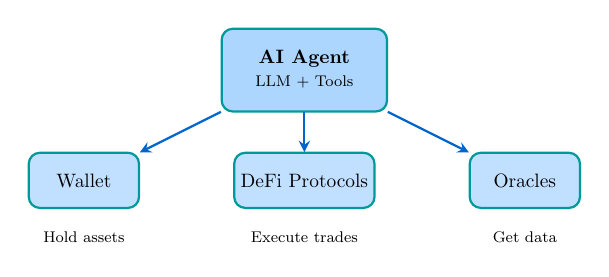
\begin{tikzpicture}[scale=0.7, transform shape]
% AI Agent
\node[blockchain, fill=dflightblue2, minimum width=3cm, minimum height=1.5cm] (ai) at (0,2) {
\begin{tabular}{c}
\textbf{AI Agent}\\
\footnotesize LLM + Tools
\end{tabular}
};

% Components
\node[blockchain, minimum width=2cm] (wallet) at (-4,0) {Wallet};
\node[blockchain, minimum width=2cm] (defi) at (0,0) {DeFi Protocols};
\node[blockchain, minimum width=2cm] (oracle) at (4,0) {Oracles};

% Connections
\draw[arrow] (ai) -- (wallet);
\draw[arrow] (ai) -- (defi);
\draw[arrow] (ai) -- (oracle);

% Actions
\node[below] at (-4,-0.8) {\footnotesize Hold assets};
\node[below] at (0,-0.8) {\footnotesize Execute trades};
\node[below] at (4,-0.8) {\footnotesize Get data};
\end{tikzpicture}
\end{center}

\vspace{3mm}
\textbf{Current Examples:}
\begin{itemize}
\item \textbf{Fetch.ai}: Autonomous economic agents
\item \textbf{Autonolas}: Agent services framework
\item \textbf{AI DAOs}: Experimental governance by AI
\end{itemize}

\begin{block}{Key Insight}
Blockchain provides the trust layer that enables AI agents to transact autonomously without human intermediation.
\end{block}
\end{frame}

% =============================================================================
% Frame 15: Open Question: The Future of Money
% =============================================================================
\begin{frame}{Open Question: The Future of Money}
\begin{center}
\textbf{What will ``money'' mean in 2035?}
\end{center}

\begin{columns}[T]
\begin{column}{0.48\textwidth}
\textbf{Continuity View:}
\begin{itemize}
\item Central banks remain dominant
\item Digital but still state-controlled
\item Private innovation at the margins
\item Regulation tightens
\item Status quo with better UX
\end{itemize}
\end{column}
\begin{column}{0.48\textwidth}
\textbf{Disruption View:}
\begin{itemize}
\item Multiple competing currencies
\item Programmable money standard
\item Algorithmic monetary policy
\item Borderless by default
\item Fundamental restructuring
\end{itemize}
\end{column}
\end{columns}

\vspace{0.5cm}
\centering
\textbf{The only certainty: more change is coming.}
\end{frame}

% =============================================================================
% Frame 16: Emerging Technologies: Zero-Knowledge Proofs
% =============================================================================
\begin{frame}{Emerging Technology: Zero-Knowledge Proofs}
\begin{block}{What Are ZK Proofs?}
Cryptographic methods to prove a statement is true without revealing the underlying data.
\end{block}

\begin{columns}[T]
\begin{column}{0.48\textwidth}
\textbf{ZK for Scaling:}
\begin{itemize}
\item \textbf{ZK-Rollups}: Bundle transactions, prove validity
\item \textbf{zkSync, StarkNet}: Production systems
\item 100x+ throughput improvements
\item Inherit L1 security
\end{itemize}
\end{column}
\begin{column}{0.48\textwidth}
\textbf{ZK for Privacy:}
\begin{itemize}
\item Prove you're over 18 without revealing age
\item Prove you have funds without showing balance
\item Regulatory-compliant privacy
\item Selective disclosure
\end{itemize}
\end{column}
\end{columns}

\vspace{3mm}
\begin{alertblock}{Why ZK Matters}
Zero-knowledge proofs may solve the privacy vs. compliance dilemma that has plagued digital finance.
\end{alertblock}
\end{frame}

% =============================================================================
% Frame 17: Emerging Technology: Account Abstraction
% =============================================================================
\begin{frame}{Emerging Technology: Account Abstraction}
\begin{block}{ERC-4337: Account Abstraction}
ERC-4337 is a standard that makes cryptocurrency wallets work more like regular app accounts, with features like password recovery. It makes blockchain accounts programmable, dramatically improving user experience.
\end{block}

\begin{columns}[T]
\begin{column}{0.48\textwidth}
\textbf{Current Problems:}
\begin{itemize}
\item Seed phrase = single point of failure
\item Gas fees in native token only
\item One transaction at a time
\item No recovery options
\end{itemize}
\end{column}
\begin{column}{0.48\textwidth}
\textbf{Account Abstraction Enables:}
\begin{itemize}
\item Social recovery (friends as backups)
\item Pay gas in any token
\item Batch multiple transactions
\item Spending limits and rules
\item Session keys for apps
\end{itemize}
\end{column}
\end{columns}

\vspace{3mm}
\begin{block}{Key Insight}
Account abstraction could make crypto as user-friendly as traditional finance while preserving self-custody.
\end{block}
\end{frame}

% =============================================================================
% Frame 18: Emerging Technology: DePIN
% =============================================================================
\begin{frame}{Emerging Technology: DePIN}
\begin{block}{Decentralized Physical Infrastructure Networks}
Using token incentives to coordinate real-world infrastructure deployment. \textbf{Note:} DePIN is still experimental with limited real-world adoption beyond niche applications.
\end{block}

\begin{columns}[T]
\begin{column}{0.55\textwidth}
\textbf{Examples:}
\begin{itemize}
\item \textbf{Helium}: Decentralized wireless networks
\item \textbf{Filecoin}: Decentralized storage
\item \textbf{Render}: Distributed GPU computing
\item \textbf{Hivemapper}: Crowdsourced mapping
\end{itemize}

\vspace{2mm}
\textbf{The Model:}
\begin{enumerate}
\item Deploy physical infrastructure
\item Earn tokens for providing service
\item Network grows through incentives
\end{enumerate}
\end{column}
\begin{column}{0.42\textwidth}
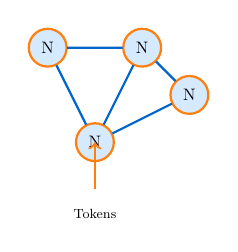
\begin{tikzpicture}[scale=0.6, transform shape]
% DePIN visualization
\node[transaction] (n1) at (0,2) {N};
\node[transaction] (n2) at (2,2) {N};
\node[transaction] (n3) at (1,0) {N};
\node[transaction] (n4) at (3,1) {N};

% Connections
\draw[thick, dfblue] (n1) -- (n2);
\draw[thick, dfblue] (n1) -- (n3);
\draw[thick, dfblue] (n2) -- (n3);
\draw[thick, dfblue] (n2) -- (n4);
\draw[thick, dfblue] (n3) -- (n4);

% Token flow
\draw[->, thick, dforange] (1,-1) -- (1,0);
\node[below] at (1,-1.3) {\footnotesize Tokens};
\end{tikzpicture}
\end{column}
\end{columns}
\end{frame}

% =============================================================================
% Frame 19: Institutional DeFi Evolution
% =============================================================================
\begin{frame}{Institutional DeFi: The Convergence Frontier}
\begin{columns}[T]
\begin{column}{0.48\textwidth}
\textbf{What Makes It ``Institutional'':}
\begin{itemize}
\item Whitelisted addresses only
\item KYC/AML verification required
\item Permissioned access layers
\item Same smart contracts underneath
\end{itemize}

\vspace{2mm}
\textbf{Examples:}
\begin{itemize}
\item Aave Arc (limited adoption)
\item Compound Treasury
\item JPM Onyx
\item Securitize
\end{itemize}
\end{column}
\begin{column}{0.48\textwidth}
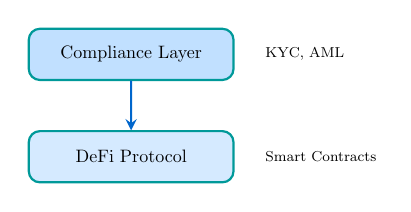
\begin{tikzpicture}[scale=0.65, transform shape]
% Two layers
\node[blockchain, minimum width=4cm, fill=dflightblue3] (compliance) at (0,2) {Compliance Layer};
\node[blockchain, minimum width=4cm, fill=dflightblue4] (defi) at (0,0) {DeFi Protocol};

% Arrow
\draw[arrow] (compliance) -- (defi);

% Side notes
\node[right] at (2.5,2) {\footnotesize KYC, AML};
\node[right] at (2.5,0) {\footnotesize Smart Contracts};
\end{tikzpicture}

\vspace{3mm}
\begin{block}{Key Difference}
Same efficiency gains, but with regulatory compliance baked in.
\end{block}
\end{column}
\end{columns}
\end{frame}

% =============================================================================
% Frame 20: Tokenized Deposits vs. Stablecoins
% =============================================================================
\begin{frame}{Tokenized Deposits vs. Stablecoins}
\begin{center}
\footnotesize
\begin{tabular}{lcc}
\toprule
\textbf{Feature} & \textbf{Tokenized Deposits} & \textbf{Stablecoins} \\
\midrule
Issuer & Commercial banks & Non-bank entities \\
Liability & Bank liability & Issuer liability \\
Insurance & FDIC insured* & No deposit insurance \\
Regulation & Bank charter & Varies by jurisdiction \\
Example & JPM Coin & USDC, USDT \\
Settlement & Private blockchain & Public/private \\
Access & Bank customers only & Permissionless \\
\bottomrule
\end{tabular}

\vspace{1mm}
{\scriptsize *FDIC = Federal Deposit Insurance Corporation (US). Similar: FSCS (UK), Einlagensicherung (EU).}
\end{center}

\vspace{2mm}
\begin{columns}[T]
\begin{column}{0.48\textwidth}
\textbf{Tokenized Deposits:}
\begin{itemize}
\item Trusted, regulated
\item Limited access
\item Existing relationships
\end{itemize}
\end{column}
\begin{column}{0.48\textwidth}
\textbf{Stablecoins:}
\begin{itemize}
\item Global, permissionless
\item Reserve transparency varies
\item DeFi composability
\end{itemize}
\end{column}
\end{columns}
\end{frame}

% =============================================================================
% Frame 21: Career Paths in Digital Finance
% =============================================================================
\begin{frame}{Career Paths in Digital Finance}
\begin{columns}[T]
\begin{column}{0.48\textwidth}
\textbf{Technical Roles:}
\begin{itemize}
\item Smart contract developer
\item Protocol engineer
\item Security auditor
\item Blockchain infrastructure
\item Data scientist (on-chain analytics)
\end{itemize}

\vspace{2mm}
\textbf{Finance Roles:}
\begin{itemize}
\item DeFi strategist
\item Digital asset trader
\item Tokenization specialist
\item Risk manager (crypto)
\end{itemize}
\end{column}
\begin{column}{0.48\textwidth}
\textbf{Hybrid Roles:}
\begin{itemize}
\item Compliance/regulatory analyst
\item Product manager (crypto)
\item Research analyst
\item Business development
\end{itemize}

\vspace{2mm}
\textbf{Emerging Roles:}
\begin{itemize}
\item AI x Crypto specialist
\item CBDC consultant
\item DAO governance expert
\item Digital identity architect
\end{itemize}
\end{column}
\end{columns}

\vspace{3mm}
\begin{block}{Key Insight}
Cross-disciplinary skills are most valuable: technical + financial + regulatory understanding.
\end{block}
\end{frame}

% =============================================================================
% Frame 22: Skills for the Future
% =============================================================================
\begin{frame}{Skills for the Future of Digital Finance}
\begin{columns}[T]
\begin{column}{0.48\textwidth}
\textbf{Technical Skills:}
\begin{itemize}
\item Solidity/smart contracts
\item Python for data analysis
\item Cryptography basics
\item API integration
\item Security fundamentals
\end{itemize}

\vspace{2mm}
\textbf{Financial Skills:}
\begin{itemize}
\item Risk management
\item Incentive analysis
\item Market microstructure
\item Valuation methods
\end{itemize}
\end{column}
\begin{column}{0.48\textwidth}
\textbf{Soft Skills:}
\begin{itemize}
\item Cross-functional communication
\item Rapid learning ability
\item Regulatory awareness
\item Critical evaluation
\end{itemize}

\vspace{2mm}
\textbf{Meta-Skills:}
\begin{itemize}
\item Separating hype from substance
\item Identifying trade-offs
\item Building mental models
\item Asking the right questions
\end{itemize}
\end{column}
\end{columns}
\end{frame}

% =============================================================================
% Frame 23: Regulatory Evolution Scenarios
% =============================================================================
\begin{frame}{Regulatory Evolution: Three Scenarios}
\begin{center}
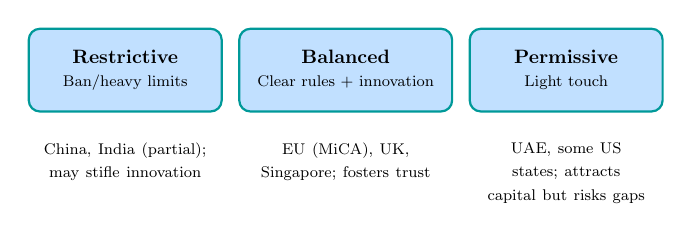
\begin{tikzpicture}[scale=0.7, transform shape]
% Three scenarios
\node[blockchain, minimum width=3.5cm, minimum height=1.5cm] (restrict) at (-4,0) {
\begin{tabular}{c}
\textbf{Restrictive}\\
\footnotesize Ban/heavy limits
\end{tabular}
};

\node[blockchain, minimum width=3.5cm, minimum height=1.5cm] (balanced) at (0,0) {
\begin{tabular}{c}
\textbf{Balanced}\\
\footnotesize Clear rules + innovation
\end{tabular}
};

\node[blockchain, minimum width=3.5cm, minimum height=1.5cm] (permissive) at (4,0) {
\begin{tabular}{c}
\textbf{Permissive}\\
\footnotesize Light touch
\end{tabular}
};

% Labels
\node[below, text width=3.3cm, align=center] at (-4,-1.2) {\footnotesize China, India (partial); may stifle innovation};
\node[below, text width=3.3cm, align=center] at (0,-1.2) {\footnotesize EU (MiCA), UK, Singapore; fosters trust};
\node[below, text width=3.3cm, align=center] at (4,-1.2) {\footnotesize UAE, some US states; attracts capital but risks gaps};
\end{tikzpicture}
\end{center}

\vspace{3mm}
\textbf{Key Regulatory Questions:}
\begin{itemize}
\item Is this a security, commodity, or new asset class?
\item Who is liable when things go wrong?
\item How do we balance innovation with consumer protection?
\item Can regulation keep pace with technology?
\end{itemize}
\end{frame}

% =============================================================================
% Frame 24: The Innovation Scorecard Revisited
% =============================================================================
\begin{frame}{The Innovation Scorecard: Your Framework}
\begin{block}{Six Questions for Any Digital Finance Innovation}
\end{block}

\begin{enumerate}
\item \textbf{PROBLEM}: What real problem does this solve, and for whom?\\
\footnotesize \textcolor{dfgray}{Red flag: Vague problem statement or only solves crypto-native problems}

\item \textbf{MECHANISM}: How does it actually work (technically and economically)?\\
\footnotesize \textcolor{dfgray}{Red flag: ``It's decentralized'' without specifics}

\item \textbf{TRADEOFFS}: What are the key tradeoffs and design choices?\\
\footnotesize \textcolor{dfgray}{Red flag: Claims of ``no tradeoffs'' or ``best of all worlds''}

\item \textbf{RISKS}: What could go wrong (technical, economic, regulatory)?\\
\footnotesize \textcolor{dfgray}{Red flag: Claims of ``no risk'' or ``guaranteed returns''}

\item \textbf{REGULATORY STATUS}: Where does it fit in the regulatory landscape?\\
\footnotesize \textcolor{dfgray}{Red flag: Regulatory arbitrage as the main strategy}

\item \textbf{WHO BENEFITS}: Who captures value, and who bears costs?\\
\footnotesize \textcolor{dfgray}{Red flag: Unclear value capture or misaligned incentives}
\end{enumerate}
\end{frame}

% =============================================================================
% Frame 25: Course Summary - The Six-Day Journey
% =============================================================================
\begin{frame}{Course Summary: The Six-Day Journey}
\begin{table}[h]
\centering
\footnotesize
\begin{tabular}{clp{8cm}}
\toprule
\textbf{Day} & \textbf{Theme} & \textbf{Key Takeaways} \\
\midrule
1 & Foundations & Money, financial system, FinTech vs. DeFi, landscape overview \\
2 & Digital Finance & Payments, API economy, data-driven finance, platform economics \\
3 & Blockchain & Cryptography, mechanics, wallets, Bitcoin vs. Ethereum \\
4 & Smart Contracts & Smart contracts, DeFi primitives, stablecoins, tokenization \& CBDCs \\
5 & Risk \& Regulation & Failures, regulation, DAO governance, privacy \& inclusion \\
6 & Future & Convergence, AI \& digital finance, synthesis framework, what's next \\
\bottomrule
\end{tabular}
\end{table}
\end{frame}

% =============================================================================
% Frame 26: Key Competencies You've Developed
% =============================================================================
\begin{frame}{Key Competencies You've Developed}
\begin{columns}[T]
\begin{column}{0.48\textwidth}
\textbf{Technical Understanding:}
\begin{itemize}
\item How blockchains achieve consensus
\item Smart contract mechanics
\item DeFi protocol design
\item Security considerations
\end{itemize}

\vspace{0.3cm}
\textbf{Economic Reasoning:}
\begin{itemize}
\item Incentive analysis
\item Market structure effects
\item Risk-return tradeoffs
\item Value capture dynamics
\end{itemize}
\end{column}
\begin{column}{0.48\textwidth}
\textbf{Regulatory Awareness:}
\begin{itemize}
\item Classification frameworks
\item Jurisdictional differences
\item Compliance requirements
\item Regulatory trajectory
\end{itemize}

\vspace{0.3cm}
\textbf{Critical Evaluation:}
\begin{itemize}
\item Separating hype from substance
\item Identifying risks and tradeoffs
\item Asking the right questions
\item Framework for any innovation
\end{itemize}
\end{column}
\end{columns}
\end{frame}

% =============================================================================
% Frame 27: The Durable Lessons
% =============================================================================
\begin{frame}{The Durable Lessons}
\begin{enumerate}
\item \textbf{No free lunch}: Every design choice involves tradeoffs. Be skeptical of claims that offer everything.

\item \textbf{Incentives matter}: Understand who profits and how. Follow the money.

\item \textbf{Technology is not enough}: Great tech fails without regulatory clarity, user adoption, and sustainable economics.

\item \textbf{Regulation follows innovation}: The rules will change. Build with regulatory evolution in mind.

\item \textbf{Decentralization is a spectrum}: Most systems are more centralized than marketed. That's not always bad.

\item \textbf{Convergence is coming}: The FinTech-DeFi divide is dissolving. Prepare for hybrid futures.

\item \textbf{Stay curious, stay skeptical}: This field moves fast. Your framework for evaluation matters more than any specific fact.
\end{enumerate}
\end{frame}

% =============================================================================
% Frame 28: Resources for Continued Learning
% =============================================================================
\begin{frame}{Resources for Continued Learning}
\begin{columns}[T]
\begin{column}{0.48\textwidth}
\textbf{News and Analysis:}
\begin{itemize}
\item The Block, CoinDesk (crypto)
\item Risk.net, American Banker (TradFi)
\item a16z crypto blog (\url{a16zcrypto.com})
\item BIS working papers
\end{itemize}

\vspace{0.3cm}
\textbf{Technical Deep Dives:}
\begin{itemize}
\item Ethereum docs
\item DeFi protocol documentation
\item Academic papers (SSRN, NBER)
\end{itemize}
\end{column}
\begin{column}{0.48\textwidth}
\textbf{Regulatory Updates:}
\begin{itemize}
\item SEC, CFTC releases
\item EU MiCA documentation
\item FSB reports
\end{itemize}

\vspace{0.3cm}
\textbf{Communities:}
\begin{itemize}
\item Protocol governance forums
\item Twitter/X crypto finance
\item Academic conferences (AFA, WFA)
\end{itemize}
\end{column}
\end{columns}

\vspace{0.3cm}
\centering
\textbf{The course ends here. Your journey continues.}
\end{frame}

% =============================================================================
% Frame 29: Discussion: Your Hypotheses
% =============================================================================
\begin{frame}{Group Discussion: Your Hypotheses}
\begin{block}{Instructions (15 minutes)}
Form small groups (3--4 students). Each group picks one open question and develops a hypothesis about how it will unfold over the next decade. Be prepared to defend your view.
\end{block}

\vspace{0.3cm}
\textbf{Structure your hypothesis:}
\begin{enumerate}
\item \textbf{Claim}: What do you think will happen?
\item \textbf{Evidence}: What current trends support this?
\item \textbf{Assumptions}: What must be true for your prediction to hold?
\item \textbf{Risks to thesis}: What could prove you wrong?
\item \textbf{Implications}: If you're right, what follows?
\end{enumerate}
\end{frame}

% =============================================================================
% Frame 30: Application: Scenario Planning Exercise
% =============================================================================
\begin{frame}{Application: Scenario Planning Exercise}
\begin{block}{Exercise: The Year is 2030}
\end{block}

\textbf{Consider these scenarios and their implications:}

\begin{columns}[T]
\begin{column}{0.48\textwidth}
\textbf{Scenario A: CBDC Dominance}
\begin{itemize}
\item Major economies launch retail CBDCs
\item Stablecoins heavily regulated
\item DeFi moves fully on-chain KYC
\item Privacy a major political issue
\end{itemize}
\end{column}
\begin{column}{0.48\textwidth}
\textbf{Scenario B: Crypto Mainstream}
\begin{itemize}
\item Bitcoin ETFs widely held
\item DeFi 2.0 with real-world integration
\item Traditional banks offer crypto services
\item Regulatory clarity achieved
\end{itemize}
\end{column}
\end{columns}

\vspace{3mm}
\textbf{Discussion Questions:}
\begin{itemize}
\item Which scenario seems more likely? Why?
\item What would you do differently in each scenario?
\item What signals would indicate which scenario is emerging?
\end{itemize}
\end{frame}

% =============================================================================
% Frame 31: Executive Summary
% =============================================================================
\begin{frame}{Executive Summary}
\begin{center}
\textbf{\Large Key Takeaways from Topic 6.4}
\end{center}

\vspace{3mm}
\begin{enumerate}
\item \textbf{Seven open questions} will shape digital finance's next decade\\
\footnotesize Interoperability, CBDCs, identity, quantum, AI, regulation, money itself

\item \textbf{No single ``winner''} is predetermined\\
\footnotesize Multiple futures possible; coexistence likely

\item \textbf{Technology continues accelerating}\\
\footnotesize ZK proofs, account abstraction, DePIN changing what's possible

\item \textbf{Careers require cross-disciplinary skills}\\
\footnotesize Technical + financial + regulatory understanding most valuable

\item \textbf{Your evaluation framework matters most}\\
\footnotesize The Innovation Scorecard works for any future development
\end{enumerate}

\vspace{3mm}
\begin{block}{The Big Idea}
Uncertainty about the future is not a weakness---it's an opportunity for those who build good mental models.
\end{block}
\end{frame}

% =============================================================================
% Frame 32: Concept Map - Course Overview
% =============================================================================
\begin{frame}{Concept Map: The Digital Finance Landscape}
\begin{center}
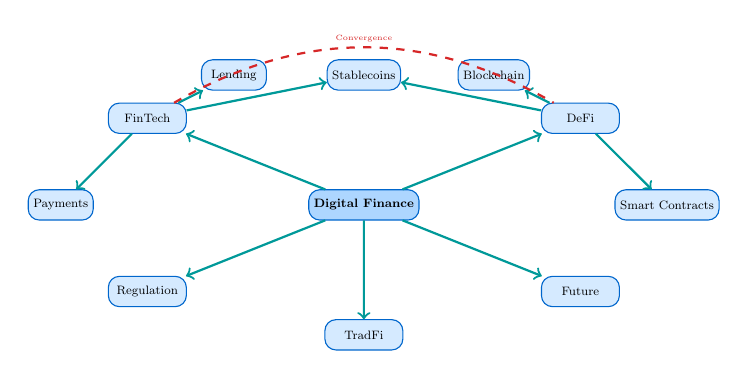
\begin{tikzpicture}[scale=0.55, transform shape,
    concept/.style={rectangle, rounded corners, draw=dfblue, fill=dflightblue4, minimum width=1.8cm, minimum height=0.7cm, font=\footnotesize},
    relationship/.style={->, thick, dfteal}]

% Central concept
\node[concept, fill=dflightblue2, minimum width=2.5cm] (df) at (0,0) {\textbf{Digital Finance}};

% Main branches
\node[concept] (fintech) at (-5,2) {FinTech};
\node[concept] (defi) at (5,2) {DeFi};
\node[concept] (tradfi) at (0,-3) {TradFi};
\node[concept] (reg) at (-5,-2) {Regulation};
\node[concept] (future) at (5,-2) {Future};

% Sub-branches
\node[concept, minimum width=1.5cm] (payments) at (-7,0) {Payments};
\node[concept, minimum width=1.5cm] (lending) at (-3,3) {Lending};
\node[concept, minimum width=1.5cm] (blockchain) at (3,3) {Blockchain};
\node[concept, minimum width=1.5cm] (smart) at (7,0) {Smart Contracts};
\node[concept, minimum width=1.5cm] (stable) at (0,3) {Stablecoins};

% Connections
\draw[relationship] (df) -- (fintech);
\draw[relationship] (df) -- (defi);
\draw[relationship] (df) -- (tradfi);
\draw[relationship] (df) -- (reg);
\draw[relationship] (df) -- (future);

\draw[relationship] (fintech) -- (payments);
\draw[relationship] (fintech) -- (lending);
\draw[relationship] (defi) -- (blockchain);
\draw[relationship] (defi) -- (smart);
\draw[relationship] (fintech) -- (stable);
\draw[relationship] (defi) -- (stable);

% Convergence arrows
\draw[dashed, thick, dfred] (fintech) to[bend left] node[above, font=\tiny] {Convergence} (defi);
\end{tikzpicture}
\end{center}

\vspace{2mm}
\textbf{Key Insight:} All components are interconnected. Understanding one requires understanding all.
\end{frame}

% =============================================================================
% Frame 33: Key Terms & Definitions I
% =============================================================================
\begin{frame}{Key Terms \& Definitions (I)}
\begin{description}
\item[Interoperability] The ability of different blockchain systems to communicate and transact with each other seamlessly.

\item[CBDC] Central Bank Digital Currency---a digital form of fiat currency issued directly by the central bank.

\item[Post-Quantum Cryptography] Cryptographic algorithms designed to resist attacks from quantum computers.

\item[Zero-Knowledge Proof] A cryptographic method to prove a statement is true without revealing the underlying data.

\item[Account Abstraction] Making blockchain accounts programmable with features like social recovery and batched transactions.
\end{description}
\end{frame}

% =============================================================================
% Frame 34: Key Terms & Definitions II
% =============================================================================
\begin{frame}{Key Terms \& Definitions (II)}
\begin{description}
\item[DePIN] Decentralized Physical Infrastructure Networks---using token incentives to coordinate real-world infrastructure.

\item[Chain Abstraction] A future state where users don't need to know or care which blockchain they're using.

\item[Institutional DeFi] DeFi protocols with added compliance layers (KYC/AML) for institutional participants.

\item[Tokenized Deposits] Bank deposits represented on blockchain, maintaining FDIC (Federal Deposit Insurance Corporation --- the US bank deposit insurance agency; similar schemes: FSCS in the UK, Einlagensicherung in the EU) insurance and bank liability status.

\item[AI Agent] An autonomous AI system capable of holding assets and executing transactions independently.

\item[Coexistence Hypothesis] The view that multiple forms of digital money (CBDCs, stablecoins, crypto) will coexist rather than one winning.
\end{description}
\end{frame}

% =============================================================================
% Frame 35: Common Misconceptions
% =============================================================================
\begin{frame}{Common Misconceptions}
\begin{columns}[T]
\begin{column}{0.48\textwidth}
\textbf{\textcolor{dfred}{Misconception}}

\vspace{2mm}
``One blockchain will win everything''

\vspace{5mm}
``CBDCs will eliminate crypto''

\vspace{5mm}
``Quantum will break all crypto soon''

\vspace{5mm}
``The future is predictable''
\end{column}
\begin{column}{0.48\textwidth}
\textbf{\textcolor{dfgreen}{Reality}}

\vspace{2mm}
Multiple chains will likely coexist with different specializations

\vspace{3mm}
Coexistence more likely; different use cases, different systems

\vspace{3mm}
Timeline is 10-30 years; migration paths exist

\vspace{3mm}
Genuine uncertainty exists; frameworks matter more than predictions
\end{column}
\end{columns}

\vspace{5mm}
\begin{alertblock}{Critical Thinking}
Be wary of anyone claiming certainty about the future. The best we can do is build good mental models and stay adaptable.
\end{alertblock}
\end{frame}

% =============================================================================
% Frame 36: Self-Assessment Question 1
% =============================================================================
\begin{frame}{Self-Assessment: Question 1}
\begin{block}{Question}
How many countries are currently exploring Central Bank Digital Currencies (CBDCs)?
\end{block}

\vspace{3mm}
\begin{enumerate}[A.]
\item 50+ countries
\item 80+ countries
\item 130+ countries
\item 200+ countries
\end{enumerate}

\vspace{5mm}
\pause
\textbf{Answer: C}

\vspace{2mm}
\textbf{Explanation:} Over 130 countries are exploring CBDCs, with China, Nigeria, and the Bahamas having already launched live implementations. This represents a significant shift in how central banks view digital currency.
\end{frame}

% =============================================================================
% Frame 37: Self-Assessment Questions 2-3
% =============================================================================
\begin{frame}{Self-Assessment: Questions 2-3}
\begin{block}{Question 2}
What is the estimated timeline for quantum computers posing a practical threat to current blockchain cryptography?
\end{block}
\textbf{Answer:} 10-30 years, with significant uncertainty. This timeline gives the industry time to migrate to post-quantum cryptographic standards.

\vspace{5mm}
\begin{block}{Question 3}
What does the course identify as the most likely future for blockchain interoperability?
\end{block}
\textbf{Answer:} The future is genuinely uncertain, with multiple possibilities: one dominant chain, chain abstraction hiding complexity, specialized chains for different uses, or traditional institutions not needing public chains at all. No single outcome is predetermined.
\end{frame}

% =============================================================================
% Frame 38: Next Steps - Continuing Education
% =============================================================================
\begin{frame}{Next Steps: Your Continued Learning}
\begin{columns}[T]
\begin{column}{0.48\textwidth}
\textbf{Immediate Actions:}
\begin{enumerate}
\item Review course materials
\item Build a project (DeFi app, analysis)
\item Follow key news sources
\item Join relevant communities
\end{enumerate}

\vspace{3mm}
\textbf{Medium-term Goals:}
\begin{itemize}
\item Deep dive into one area
\item Contribute to open-source
\item Attend conferences/meetups
\item Consider certifications
\end{itemize}
\end{column}
\begin{column}{0.48\textwidth}
\textbf{Certifications to Consider:}
\begin{itemize}
\item CFA (traditional finance)
\item CAIA (alternative investments)
\item Blockchain developer certs
\item Compliance certifications
\end{itemize}

\vspace{3mm}
\textbf{Advanced Study:}
\begin{itemize}
\item Master's in FinTech
\item Specialized courses (DeFi, ML)
\item Research opportunities
\item Industry internships
\end{itemize}
\end{column}
\end{columns}

\vspace{3mm}
\begin{block}{Remember}
The field changes faster than any curriculum. Your ability to learn and adapt matters more than any credential.
\end{block}
\end{frame}

% =============================================================================
% Frame 39: Resources & References
% =============================================================================
\begin{frame}{Resources \& References}
\textbf{Key Publications:}
\begin{itemize}
\item BIS: ``The Future of the Monetary System'' (Annual Economic Report)
\item Atlantic Council: CBDC Tracker (\url{atlanticcouncil.org/cbdctracker})
\item NIST: Post-Quantum Cryptography Standards
\end{itemize}

\vspace{3mm}
\textbf{Research Sources:}
\begin{itemize}
\item SSRN FinTech and DeFi research papers
\item Ethereum Foundation research blog
\item a16z State of Crypto reports
\end{itemize}

\vspace{3mm}
\textbf{Industry Resources:}
\begin{itemize}
\item Messari, Delphi Digital (research reports)
\item Chainalysis (on-chain analytics)
\item Protocol governance forums (Compound, Aave, etc.)
\end{itemize}

\vspace{3mm}
\textbf{Course Materials:} All slides and notebooks available on the course website.
\end{frame}

% =============================================================================
% Frame 40: Questions? + Course Completion
% =============================================================================
\begin{frame}{Congratulations!}
\begin{center}
\textbf{\Large Course Complete}

\vspace{5mm}
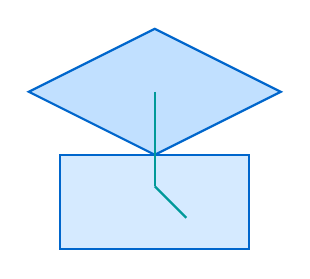
\begin{tikzpicture}[scale=0.8, transform shape]
% Graduation cap
\draw[thick, dfblue, fill=dflightblue4] (-1.5,0) -- (1.5,0) -- (1.5,1.5) -- (-1.5,1.5) -- cycle;
\draw[thick, dfblue, fill=dflightblue3] (0,1.5) -- (-2,2.5) -- (0,3.5) -- (2,2.5) -- cycle;
\draw[thick, dfteal] (0,2.5) -- (0,1);
\draw[thick, dfteal] (0,1) -- (0.5,0.5);
\end{tikzpicture}

\vspace{5mm}
\textbf{\Large ``The best way to predict the future\\is to invent it.''}\\[0.3cm]
\normalsize --- Alan Kay

\vspace{5mm}
You now have the tools to not just observe digital finance,\\
but to \textbf{critically evaluate}, \textbf{thoughtfully participate},\\
and perhaps \textbf{help shape} its future.

\vspace{5mm}
\textbf{Thank you for your engagement throughout the course.}

\vspace{3mm}
\textbf{Contact:} joerg.osterrieder@gmail.com
\end{center}
\end{frame}

\end{document}
